\section{Waves}
\subsection{General properties of waves}

Waves are through which energy is transferred without transfer of matter.

\begin{center}
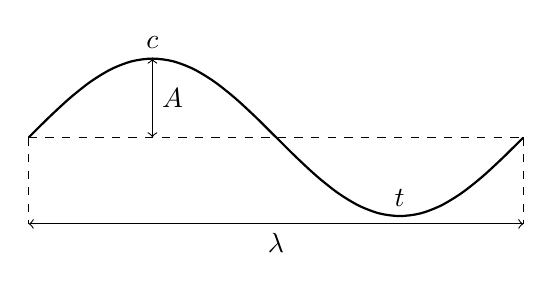
\begin{tikzpicture}

    % Draw the wave
	\draw[thick, domain=0:6.28, smooth, variable=\x] 
        plot ({\x}, {sin(\x r)});
        
    % Label for the wave
	\draw[<->] (0, -1.1) -- (6.28, -1.1) node[midway, below]{$\lambda$};

    % Amplitude arrow
    \draw[<->] (1.57,0) -- (1.57,1) node[midway, right] {$A$};
	\draw (1.57, 1) node[above] {$c$};
	\draw (1.57*3, -1) node[above] {$t$};

	\draw[dashed] (0, 0) -- (0, -1.1);
	\draw[dashed] (6.28, 0) -- (6.28, -1.1);
	\draw[dashed] (0, 0) -- (6.28, 0);
    
\end{tikzpicture}
\end{center}
Above is a diagram of a typical wave. It shows some characteristics of all waves. The wavelength
of a wave is the distance between two adjacent identical points in the wave, denoted by $\lambda$. The
amplitude of a wave is the maximum height from equilibrium position (the dotted line) of the wave,
denoted by $A$. The highest and lowest points of a wave are called the waves crest and trough
respectively, shown in the above diagram as $c$ and $t$ respectively. Every wave propagates, i.e.,
covers distance per unit time, known as its speed or the wave speed, denoted $v$. Never is there
only one wave being produced, multiple waves are usually produced simultaneously. The crests
and troughs of all these waves form lines called wavefronts.

Frequency, $f$ is the number of wavelengths of a wave that pass a point per unit time. Its unit
is Hertz (Hz), which is equivalent to \SI{}{s^{-1}} (per second). The amplitude, $A$ of the
wave can also be said to be the maximum distance of a particle from the mean position.

Wave speed can be found using the following equation:
$$ v = f\lambda$$

Waves can be of two types, transverse and longitudinal. The former is those where the direction
of wave propagation is perpendicular/normal to the direction of particle oscillation.
Water waves, electromagnetic waves and seismic secondary waves are all transverse waves.
In the latter,
direction of wave propagation is parallel to that of particle oscillation.  Examples include
sound waves and seismis primary waves.

When waves arrive at a plane surface, they are reflected. A change in speed of a wave causes
its direction of propagation to change, which is known as refraction of the wave. When it 
travels through a gap, it is diffracted. Diffraction may also occur as a result of a wave
passing beside an edge.

When waves pass through a barrier in which there is a gap whose width is greater than the wave's
wavelength, diffraction's effect is not quite pronounced. The effect is most pronounced when the
gap equals the wave's $\lambda$. When the gap is much smaller than the wave's wavelength, the
wave does not pass through at all.

When waves pass by an edge, the angle of diffraction of the waves is directly related to the 
resulting angle of diffraction.

\subsection{Light}
\subsubsection{Reflection of light}
Reflection is the change of direction of a wave when it strikes a plane surface without passing
through it. Light is reflected by shiny surfaces such as mirrors.

\begin{center}
\begin{tikzpicture}

    % Draw the horizontal surface
    \draw[thick] (-2,0) -- (6,0) node[right] {Surface};

    % Draw the normal to the surface at the point of contact
    \draw[dashed] (2,-2) -- (2,3);

    % Draw the incident ray
	\draw[-, thick]  (2,0) -- (-1,2) node[left] {Incident ray};

    % Draw the reflected ray
    \draw[->, thick] (2,0) -- (5,2) node[right] {Reflected ray};

    % Draw the angle of incidence
    \node at (1.55,1) {$i$};

    % Draw the angle of reflection
    \node at (2.45,1) {$r$};
\end{tikzpicture}
\end{center}

The normal of a surface is an imaginary line that is perpendicular to the surface. When waves are
reflected, an angle of incidence is formed between the incident ray and the normal of the surface
of reflection. This incidence angle is called $i$. The reflected ray of the wave also forms a
reflected angle with the normal of the surface, denoted as $r$. In case of reflection $i = r$.

\subsubsection{Refraction of light}
In the case when the incident ray is not reflected off rather it passes into the surface, 
refraction occurs. The reflected ray is now called the refracted ray and the reflected angle the
refracted angle. The extent of refraction depends on the material's refracting index, $n$.

The refractive index of a material can be found by:
$$ n = \frac{\sin{i}}{\sin{r}} = \frac{c_i}{c_r} $$
where $c_1$ is the speed of wave in incidence medium and $c_2$ is that in refracted medium.

The critical angle of a material is that beyond which total internal reflection of a wave will
occur and at which the incidence re-emergent ray is at \SI{90}{\degree} to the normal. Hence,
$$ n = \frac{1}{\sin{c}} $$
where $c$ is the critical angle.

Optical fibres consist of fibres whose interiors are lined with glass like substances. They are 
used to transmit information at light speed, as when light travels through these optical fibres,
the angle of incidence of each ray is always greater than critical angle and hence no light is
lost to refraction, no information is lost either.

\subsubsection{Thin lenses}
Lenses can be of two types: converging and diverging lenses.

TODO: Diagrams.

Understand that,
$$ \textrm{linear magnification} = \frac{\textrm{image length}}{\textrm{object length}} $$

\subsubsection{Dispersion of light}
White light, when it passes through a glass prism, due to differences in its component colours,
frequencies, wavelengths, will disperse into its 7 component colours. The seven component colours
are violet, indigo, blue, yellow, orange and red, in sequence of decreasing frequency and 
increasing wavelength.

\subsection{Electromagnetic spectrum}

Electromagnetic waves are a waves which all have a speed of $\num{3e8}$ \SI{}{m/s} in vacuum.
It is a spectrum of waves as each wave differs by its wavelength and frequency, the two being
inversely related.
